\documentclass[openany]{book}
% !TeX TXS-program:compile = txs:///pdflatex/[--shell-escape]
\usepackage{macros}
\usepackage{notes}

%% PICTURES DIRECTORY %%
\graphicspath{{C:/Users/Michael/Pictures/}}
\graphicspath{{C:/Users/Michael/Pictures/MATH113}}

% REDEFINING CHAPTER FORMATTING %
\newif\iftoc\titleformat{\chapter}[display]{\cabin}{}{2in}{
	\raggedleft
	\iftoc
	\vspace{2in}
	\else
	{\LARGE\textsc{Week}~{\cantarell\thechapter}} \\
	\fi
	\Huge\scshape\bfseries
}[\vspace{-20pt}\rule{\textwidth}{0.1pt}\vspace{0.0in}]
\titlespacing{\chapter}{0pt}{
	\iftoc
	-100pt+1in
	\else
	-130pt+1in
	\fi
}{0pt}

%% RENEW TITLE PAGE %%
\renewcommand{\mytitle}[2]{%
	\title{#1}
	\author{Michael Pham}
	\date{#2}
	\maketitle
	\newpage
	\mytoc
	\newpage
}

\begin{document}
\mytitle{MATH 113: Introduction to Abstract Algebra}{Fall 2024}

\chapter{Introductions}
\section{Lecture -- 8/29/2024}
\subsection{What is Algebra?}
To begin with, when we see the word ``algebra", we think of equations.

\begin{example}[Where Algebra Comes In]
	Suppose we were asked to solve the following equation:
	\begin{equation*}
		x(x+y) = yx
	\end{equation*}

	A typical way of solving it would be as follows:
	\begin{align}
		x(x+y) &= yx \\
		x^{2} + xy &= yx \\
		x^{2} &= yx + (-1)(xy) \\
		x^{2} &= yx + (-1)(yx) \\
		x^{2} &= 0 \\
		x &= 0
	\end{align}

	When going through this basic example, we note in (1.4), we are assuming that $xy = yx$; this is where the idea of ``algebra" actually comes into play! We are assuming here that we have commutativity.
	
	Similarly, in (1.6), we are assuming that $x^{2} = 0 \implies x = 0$. Once again, we are making assumptions that these properties hold and we are working with some underlying structure in-place.
	
	This is algebra.
\end{example}

\begin{warn}
	We note that $xy = yx$ doesn't always hold! For example, let us look at matrix multiplication:
	\begin{equation*}
		\begin{bmatrix}
			1 & 0 \\
			0 & 0
		\end{bmatrix}
		\begin{bmatrix}
			0 & 1 \\ 0 & 1
		\end{bmatrix} =
		\begin{bmatrix}
			0 & 2 \\ 0 & 0
		\end{bmatrix}
	\end{equation*}

	However, we see that if we multiplied them in the other order, we would instead get:
	\begin{equation*}
		\begin{bmatrix}
			0 & 1 \\ 0 & 1
		\end{bmatrix}\begin{bmatrix}
		1 & 0 \\
		0 & 0
	\end{bmatrix} =
		\begin{bmatrix}
			0 & 0 \\ 0 & 0
		\end{bmatrix}
	\end{equation*}
\end{warn}

\begin{warn}
	We also note that $x^{2} = 0 \implies x = 0$ isn't true! Again, we can look towards matrices for a counterexample:
	\begin{equation*}
		\begin{bmatrix}
			0 & 1 \\ 0 & 0
		\end{bmatrix}\begin{bmatrix}
		0 & 1 \\ 0 & 0
	\end{bmatrix} = \begin{bmatrix}
	0 & 1 \\ 0 & 0
\end{bmatrix}^{2} = \begin{bmatrix}
	0 & 0 \\ 0 & 0
\end{bmatrix}
	\end{equation*}
\end{warn}

Now, we look at the following example:
\begin{example}[Sneak Peek into Groups]
	Let us consider the following equation: $x + a = b$.
	
	To solve for $x$, we can proceed as follows:
	\begin{align*}
		x + a &= b && \\
		(x + a) + (-a) &= b + (-a) && \text{\textit{(Inverse)}} \\
		x + (a + (-a)) &= b + (-a) && \text{\textit{(Associativity)}} \\
		x + 0 &= b + (-a) && \\
		x &= b + (-a) && \text{\textit{(Identity)}}
	\end{align*}

	In each line, we note the property needed to make the step. We also note here that this foreshadows the concept of ``groups" -- sets with some operation satisfying the three properties mentioned above.
\end{example}

\begin{example}[Some Counterexamples]
	We can think of some basic examples of sets which don't satisfy (at least one of) the properties:
	\begin{itemize}
		\item $(\NN, +)$ doesn't satisfy inverses.
		\item $(\NN, \times)$ doesn't satisfy inverses.
		\item $(\RR^{n \times n}, \times)$ doesn't satisfy associativity.
	\end{itemize}
\end{example}

\subsection{Some Proofs Techniques}
Going into this course, writing proofs will play an important part. As such, it is important to recall certain proof techniques:
\begin{itemize}
	\item Proof by Contradiction
	\begin{itemize}
		\item For example, we can use this to prove that $\sqrt{2}$ is irrational.
	\end{itemize}
	\item Proof by Cases
	\begin{itemize}
		\item For example, we can use this to prove that $x(x+1)$ is even.
	\end{itemize}
	\item (Strong) Induction
	\begin{itemize}
		\item For example, we can use this to prove that $\sum_{i=1}^{n} = \frac{n(n+1)}{2}$.
	\end{itemize}
\end{itemize}

\section{Lecture -- 8/30/2024}
\subsection{Administrivia}
\begin{miscbox}{Textbooks Used}
	For the purposes of this course, we will mostly be working with Judson's \textit{Abstract Algebra: Theory and Applications}. The book will be referred to as [Open].
	
	Another very good textbook that will sometimes be referenced is Dummit and Foote's \textit{Abstract Algebra}. This will be referred to by [DF].
\end{miscbox}

We also note that any schedule provided for the timeline of topics is approximate; pacing may vary!

\subsection{Pre-Examples}
In this lecture, we will be looking at the concept of equivalence classes.

\begin{example}[The Rationals $\QQ$]
	To begin with, let us consider the set $\QQ$ and how we can describe the elements in it.
	
	A naive approach is to simply state that for $q \in \QQ$, we can write it such that $p \in \ZZ$ and $q \in \NN$.
	
	However, this doesn't fix a relatively important issue: with this approach, $\frac{1}{2} \neq \frac{2}{4}$, despite us treating them as being the same.
	
	This is where equivalence classes will come into play.
\end{example}

\subsection{Sets}
\begin{defn}[Set]
	We define a set as a collection of elements.
	
	A set $X$ can be written in the following ways:
	\begin{align*}
		X &= \brc{x_1, \ldots, x_n} \\
		&= \brc{x_i} \\
		&= \brc{x : \varphi(x)}
	\end{align*}
\end{defn}

\begin{defn}
	For sets $X, Y$, we let $X \times Y$ to be the Cartesian product defined as:
	\begin{equation*}
		X \times Y = \brc{(x, y) : x \in X \land y \in Y}.
	\end{equation*}
\end{defn}

We note that $(x, y)$ is an ordered pair. That is, $(x, y) \neq (y, x)$.

\subsection{Maps}
\begin{defn}[Map]
	A map $f: X \rightarrow Y$ is a rule that assigns a unique element of $Y$ to each element of $X$.
\end{defn}
\begin{warn}
	It is important to note that a map \textbf{must} assign every element in the domain to some element in the codomain. And we note that it must be a \textit{unique} element as well; we can't map one element in the domain to multiple in the codomain.
\end{warn}
\subsubsection{Types of Maps}
\begin{defn}[Surjectivity]
	We say that a map $f: X \rightarrow Y$ is surjective iff for all $y \in Y$, there exists some $x \in X$ such that $f(x) = y$.
\end{defn}

\begin{defn}[Injectivity]
	We say that a map $f : X \rightarrow Y$ is injective iff for $x_1, x_2 \in X$, if $f(x_1) = f(x_2)$, then $x_1 = x_2$.
	
	Similarly, we can take the contrapositive and say that if $x_1 \neq x_2$, then $f(x_1) \neq f(x_2)$.
\end{defn}

\begin{defn}[Bijectivity]
	We say that a map $f: X \rightarrow Y$ is bijective iff it is both injective and surjective.
\end{defn}

\subsection{Equivalence Relations}
\begin{defn}[Equivalence Relation]
	We define an equivalence relation $R$ (or $\sim$) on a set $X$ to be a subset $R \subseteq X \times X$ such that it has the following properties:
	\begin{itemize}
		\item Reflexivity: $\forall x (\ang{x, x} \in R)$
		\item Symmetry: $\forall x \forall y(\ang{x, y} \in R \implies \ang{y, x} \in R)$.
		\item Transitivity: $\forall x\forall y \forall z (\ang{x,y} \in R \land \ang{y, z} \in R \implies \ang{x, z} \in R)$.
	\end{itemize}
\end{defn}

We say that $x \sim y$ iff $\ang{x, y} \in R$.

\begin{defn}[Equivalence Class]
	We say that an equivalence class of $x \in X$ is a set defined as follows:
	\begin{equation*}
		[x] = \brc{y \in X : (x, y) \in R} = \brc{y \in X : x \sim y}
	\end{equation*}
\end{defn}

\begin{defn}[Quotient]
	A quotient of $X$ by an equivalence relation $R$ is $X/\sim$, which is the set of all $R$-equivalence classes.
\end{defn}

\begin{example}[Ages on Humans]
	Suppose that we are looking at the set of all human beings. We denote this by $S$.
	
	Now, one way to partition them up is to group them into their ages. Then, we can think of each age as being an equivalence class, containing all the human beings that fall under said age. Furthermore, the set of all of the ages can be thought of as the quotient.
\end{example}

\chapter{Second Week Woes}
\section{Lecture -- 9/4/2024}
\subsection{Warm Up}
\begin{hw}[Types of Maps]
	Suppose we have the following map:
	\begin{center}
		\begin{tikzpicture}
			\node[draw, ellipse, minimum width = 2cm, minimum height = 5cm, label = above left:$A$] (A) at (0, 0) {};
			
			\node[draw, ellipse, minimum width = 1cm, minimum height = 3cm, label = above left:$B$] (B) at (0, -0.75) {};
			
			\node (p1) at (0, 1.5) {};
			\fill (0, 1.5) circle (0.05);
			
			\node (p2) at (0, 0) {};
			\fill (0, 0) circle (0.05);
			
			\node (p3) at (0, -1.5) {};
			\fill (0, -1.5) circle (0.05);
			
			
			\node[draw, ellipse, minimum width = 2cm, minimum height = 5cm, label = above right:$C$] (C) at (5, 0) {};
			
			\node[draw, ellipse, minimum width = 1cm, minimum height = 3cm, label = above right:$D$] (D) at (5, -0.75) {};
			
			\node (p4) at (5, 1.5) {};
			\fill (5, 1.5) circle (0.05);
			
			\node (p5) at (5, 0) {};
			\fill (5, 0) circle (0.05);
			
			\node (p6) at (5, -1.5) {};
			\fill (5, -1.5) circle (0.05);
			
			\draw[->] (p1) -- (p5);
			\draw[->] (p2) -- (p5);
			\draw[->] (p3) -- (p6);
		\end{tikzpicture}
	\end{center}

	Based off of this graph, suppose we had the following maps:
	\begin{enumerate}
		\item $f : A \rightarrow C$.
		\item $f : A \rightarrow D$.
		\item $f : B \rightarrow C$.
		\item $f : B \rightarrow D$.
	\end{enumerate}

	Now, we want to determine whether the maps are injective, surjective, bijective, or none.
\end{hw}
\begin{solution}
	For $f : A \rightarrow C$, we see that since two elements are mapped to the same element in $D$, it isn't an injection. Furthermore, not all elements of $C$ are being mapped to by $f$, so it is not a surjection either. Thus, it is \textbf{neither}.
	
	For $f : A \rightarrow D$, we see that it isn't injective due to the same reason provided previously. However, all elements of $D$ are mapped to by some element of $A$. Thus it is a \textbf{surjection}.
	
	For $f: B \rightarrow C$, we see that not all elements of $C$ are mapped to by an element in $B$. However, each element in $B$ map to a different element in $C$. Thus, it is an \textbf{injection}.
	
	For $f : B \rightarrow D$, we see that it's still injective by the previous reason. However, since all elements of $D$ are being mapped to by some element in $B$, it is surjective as well. Thus, it is a \textbf{bijection}.
\end{solution}

\subsection{$\ZZ$ and $\ZZ/n\ZZ$}
\subsubsection{Algebraic Structures}
First, let us provide some notation. When we have something like $\pr{\ZZ, +}$ or $\pr{\ZZ, \times}$, these are algebraic structures. This is simply a set -- so in this case, $\ZZ$ -- equipped with some operation ($+$ and $\times$ in our examples).

\begin{warn}
	Note that $\ZZ$ is a countably infinite set.
\end{warn}

\subsubsection{$\pr{\ZZ, +}$ versus $\pr{\ZZ, \times}$}
We can do a comparison of the two structures as follows:
\begin{multicols}{2}
	$(\ZZ, +)$:
	\begin{itemize}
		\item Identity: $0$.
		\begin{itemize}
			\item $a + 0 = a$.
		\end{itemize}
		\item Inverse: $(-a)$
		\begin{itemize}
			\item $a + (-a) = 0$
		\end{itemize}
		\item Commutativity
		\begin{itemize}
			\item $a + b = b + a$
		\end{itemize}
	\end{itemize}
	
	$(\ZZ, \times)$:
	\begin{itemize}
		\item Identity: $1$.
		\begin{itemize}
			\item $a \times 1 = a$.
		\end{itemize}
		\item Inverse: None.
		\item Commutativity
		\begin{itemize}
			\item $a \times b = b \times a$
		\end{itemize}
	\end{itemize}
\end{multicols}

\subsection{Generators}
When we write $\ZZ = \ang{1}$, this is denoting that $1$ generates $\pr{\ZZ, +}$ as a group.

To make this more concrete, we note that for all $n \in \ZZ$, we can write $n$ as a sum of $n$ $1$'s (or $(-1)$'s).

We note that for $\pr{\ZZ, \times}$, we can generate it by considering the set of all prime numbers.

By the Fundamental Theorem of Arithmetic, we note htat for all $n \in \ZZ$, we can write it as follows:
\begin{equation*}
	n = (\pm 1) \prod_{i=1}^{m} p_i^{a_i},
\end{equation*}
where $m \in \NN$, $p_i$ is some prime, and $a_i \in \NN$.

\begin{thm}[Number of Primes]
	There are infinitely many primes.
\end{thm}
\begin{proof}
	We can proceed by contradiction.
	
	Let us suppose that there are finitely many primes. Then, suppose that we have $k$ primes. We can thus list them $p_1, \ldots, p_k$.
	
	Now, let us consider the product $P = p_1 \cdots p_k$. Then, let us denote $q = P + 1$. By construction then, we note that $q$ is not divisible by any of our $p_1, \ldots, p_k$.
	
	From here, we have two cases:
	\begin{enumerate}
		\item $q$ is a prime number.
		\item $q$ is not a prime number.
	\end{enumerate}

	In the first case, if $q$ is prime, then there is a contradiction. Thus, it follows that there must be infinitely many primes.
	
	In the second case, we note that if $q$ isn't prime, there must exist some prime factor $p$ which divides $q$. However, by construction, this $p$ cannot be in our list of primes, and thus we have a contradiction.
	
	Therefore, we conclude that there are infinitely many primes.
\end{proof}

\subsection{What is $\ZZ / n \ZZ$?}
We say that $\ZZ / n \ZZ$ is the remainder of dividing any $m \in \ZZ$ by $n$ (where $n$ is some natural number).

With this in mind, let us provide the following definition:
\begin{defn}[Divides By]
	We say that $n \mid a$ if $\pr{\exists x \in \ZZ}\pr{a = xn}$.
	
	More concretely, we note that our remainder is equal to zero in our division algorithm:
	\begin{equation*}
		a = xn + r.
	\end{equation*}
\end{defn}

Now, we give the following equivalence relation for $\ZZ$:
\begin{defn}
	$\forall a, b \in \ZZ$, we say that $a \sim b$ iff $n \mid (a - b)$.
\end{defn}

Before we proceed further, we should actually confirm if this defines an equivalence relation or not:
\begin{enumerate}
	\item First, for reflexivity, we see that $(a - a) = 0$. And trivially, we see that $n \mid 0 \implies a \sim a$.
	Thus, we see that, indeed, $n \mid (a - a)$; $a \sim a$.
	\item Next, symmetry. Suppose that $a \sim b$. Then, this means that there exists some $x \in \ZZ$ such that $xn = a - b$. This means then that $-xn = b - a$, and $-x \in \ZZ$ as well. Thus, indeed, we see that $n \mid (b - a) \implies b \sim a$.
	\item Finally, for transitivity, suppose that $a \sim b$ and $b \sim c$. Then, we note that there exists some $x$ and $y$ such that $a - b = xn$ and $b - c = yn$. Then, $(a - b) + (b - c) = xn + yn$. This becomes $a - c = n(x + y)$, and by closure of $\ZZ$ under addition, we note that, indeed, $n \mid (a - c) \implies a \sim c$ as desired.
\end{enumerate}

Thus, we see that we do indeed have an equivalence relation.

\subsubsection{Equivalence Classes}
Now, we look at the equivalence classes of $\ZZ$ under the given equivalence relation. We observe that for $n = 5$, we have:
\begin{align*}
	[0] &= \brc{\ldots, -5, 0, 5, \ldots} \\
	[1] &= \brc{\ldots, -4, 1, 6, \ldots} \\
	&\vdots \\
	[4] &= \brc{\ldots, -1, 4, 9, \ldots}
\end{align*}

And we note that $\cdots = [-5] = [0] = [5] = \cdots$. The same logic applies to the other equivalence classes.

And with all of this, we can finally define $\ZZ / n \ZZ$ as the set of equivalence classes for $n$ under the equivalence relation $\sim$. 

\section{Required Reading -- 9/6/2024}
\subsection{Symmetries}
A natural way of thinking about groups is to consider symmetries.

\begin{defn}[Symmetry]
	We define a symmetry of a geometric figure to be a rearrangement of the figure which preserves the arrangement of its sides and vertices, along with its distances and angles.
\end{defn}

\begin{defn}[Rigid Motion]
	A map from the plane to itself preserving the symmetry of an object is called ``rigid motion."
\end{defn}
\newpage
%\begin{center}
%	\begin{tikzpicture}
%		\node[label=above left:A] (a1) at (0, 2) {};
%		\node[label=above right:B] (b1) at (4, 2) {};
%		\node[label=below right:C] (c1) at (4, 0) {};
%		\node[label=below left:D] (d1) at (0, 0) {};
%		\draw (a1) -- (b1) -- (c1) -- (d1) -- (a1);
%	\end{tikzpicture}
%\end{center}
\begin{figurebox}[]{Rigid Motions of Rectangle}
	\centering\includegraphics[]{m113-rects}
\end{figurebox}

We observe from the figure above how while the transformations provided preserves the orientation of the rectangle and the relationships among it vertices, if we did something like a $90^{\circ}$ rotation, it wouldn't be considered a symmetry.

Let us look at a different examples with triangles:

\begin{figurebox}[]{Symmetries of a Triangle}
	\centering\includegraphics[]{m113-tris}
\end{figurebox}

First, note that we can encode the transformation using a matrix. Let us look at the following:
\begin{equation*}
	\begin{pmatrix}
		A & B & C \\ C & B & A
	\end{pmatrix}
\end{equation*}

We observe that this is telling us that we are mapping corner $A$ to $C$, $B$ to $B$, and $C$ to $A$.

\begin{defn}[Permutation]
	A permutation of a set $S$ is some bijection $\pi : S \to S$.
\end{defn}

An interesting thing to note, which is shown in the figure, is that every permutation (of which there are $3! = 6$) corresponds to some symmetry of our triangle.

Now, a question to ask would be what happens if we combine two different motions for our triangle? For example, let us consider $\mu_1 \rho_1$ (that is, we apply $\rho_1$ onto the triangle, followed by $\mu_1$).

Well, we can proceed as follows:
\begin{align*}
	\mu_1\rho_1(A) &= \mu_1(B) \\
	&= C \\
	\mu_1\rho_1(B) &= \mu_1(C) \\
	&= B \\
	\mu_1\rho_1(C) &= \mu_1(A) \\
	&= A
\end{align*}

Thus, we note that we get the same transformation as if we simply did $\mu_2$. Note that this is pretty intuitive that composing permutations will result in some new transformation, since they are just bijections from $S$ onto itself.

\begin{warn}
	We note that we are composing functions when looking at multiple permutations being applied. Thus, we read from right to left.
\end{warn}

\subsection{Definitions and Examples}
\subsubsection{Groups}
As hinted at previous, the integers mod $n$ and the symmetries of a triangle (or rectangle) are all examples of what we call a ``group."

\begin{defn}[Binary Operation]
	A binary operation (sometimes called a law of composition) on a set $G$ is a function $G \times G \rightarrow G$ which assigns to each pair $(a, b) \in G \times G$ a unique element $a \circ b$ (or $ab$) in G. This is called the composition of $a$ and $b$.
\end{defn}

\begin{defn}[Group]
	A group $(G, \circ)$ is defined then as a set $G$ together with some binary operation $(a, b) \mapsto a \circ b$ which satisfies the following three properties:
	\begin{itemize}
		\item Associativity: $(a \circ b) \circ c = a \circ (b \circ c)$, for all $a,b,c \in G$.
		\item Identity: There exists some identity element $e \in G$ such that $a \circ e = a = e \circ a$, for all $a \in G$.
		\item Inverse: For every element $a \in G$, there exists some inverse $a^{-1}$ such that $a \circ a^{-1} = e = a^{-1} \circ a$. 
	\end{itemize}
\end{defn}

\begin{defn}[Abelian]
	We note that if a group happens to satisfy commutativity (that is, $a \circ b = b \circ a$), then the group is an abelian group. They are also referred to as being commutative groups.
\end{defn}

\subsubsection{Examples}
\begin{example}[The Integers $\ZZ$]
	First, we note that $(\ZZ, +)$ forms a group (as seen previously). And in fact, it is actually an abelian group.
	
	On the other hand, $\pr{\ZZ, \times}$ doesn't, as it fails the inverse check.
	
	Similarly, $\ZZ / n \ZZ$ also forms a(n abelian) group. It is often convenient to describe a group in terms of an addition or multiplication table; these are called Cayley tables, specifically.
\end{example}

\begin{example}[Matrices]
	We denote $\mathbb M_2 (\RR)$ to be the set of all $2 \times 2$ matrices. Then, let $GL_2(\RR)$ to be the subset of $\mathbb M_2(\RR)$ which contains only invertible matrices.
	
	Then, this means that $GL_2(\RR)$ is in fact a (nonabelian) group under matrix multiplication. 
	
	We note that matrix multiplication is associative. Furthermore, we have the identity matrix:
	\begin{equation*}
		I = \begin{bmatrix}
			1 & 0 \\ 0 & 1
		\end{bmatrix}
	\end{equation*}

	And for every matrix $A$, we have an inverse $A^{-1}$ defined as:
	\begin{equation*}
		A^{-1} = \frac{1}{ad-bc}\begin{bmatrix}
			d & -b \\ -c & a
		\end{bmatrix}
	\end{equation*}
\end{example}

\subsection{Basic Properties of Groups}
\begin{prop}
	The identity element in $G$ is unique.
\end{prop}
\begin{proof}
	Suppose for the sake of contradiction that the identity element isn't unique. Then, there exists $e, e'$ (with $e \neq e'$) such that $eg = g = ge$ and $e'g = g = ge'$, for all $g \in G$.
	
	Then, we observe the following: if $e$ is the identity element, then we have that:
	\begin{align*}
		ee' &= e'
	\end{align*}

	However, since $e'$ is also the identity element, we see then that:
	\begin{align*}
		ee' &= e
	\end{align*}

	In other words, we have:
	\begin{align*}
		ee' = e = ee' = e'
	\end{align*}

	In other words, we have $e = e'$; thus, the identity element is in fact unique.
\end{proof}

Similarly, we have the following proposition:
\begin{prop}
	For any element $g \in G$, its inverse $g^{-1}$ is unique.
\end{prop}

The proof for this is similar to the one for proving uniqueness of the identity.

\begin{prop}
	Let $G$ be a group. If $a, b \in G$, then $(ab)^{-1} = b^{-1}a^{-1}$.
\end{prop}
\begin{proof}
	Suppose that $G$ is a group, and we have $a, b \in G$.
	
	Then, we observe the following:
	\begin{align*}
		(ab)(b^{-1}a^{-1}) &= a(bb^{-1})a^{-1} \\
		&= a(ea^{-1}) \\
		&= aa^{-1} \\
		&= e \\
		\\
		(b^{-1}a^{-1})(ab) &= b^{-1}(a^{-1}a)b \\
		&= b^{-1}(eb) \\
		&= b^{-1}b \\
		&= e
	\end{align*}

	Then, since inverses are unique, we observe then that $(ab)^{-1} = b^{-1}a^{-1}$.
\end{proof}

\begin{prop}
	Let $G$ be a group. Then, for any $a \in G$, we have that $(a^{-1})^{-1} = a$.
\end{prop}
\begin{proof}
	We proceed as follows:
	\begin{align*}
		(a^{-1})(a^{-1})^{-1} &= e \\
		a(a^{-1})(a^{-1})^{-1} &= ae \\
		(aa^{-1})(a^{-1})^{-1} &= a \\
		e(a^{-1})^{-1} &= a \\
		(a^{-1})^{-1} &= a
	\end{align*}
\end{proof}

\begin{prop}
	Let $G$ be a group, and $a, b \in G$. Then, the equations $ax = b$ and $xa = b$ have unique solutions.
\end{prop}
\begin{proof}
	Let us suppose that $ax = b$. Then, to show that a solution indeed exists, we proceed as follows:
	\begin{align*}
		a^{-1}(ax) &= a^{-1}b \\
		(a^{-1}a)x &= a^{-1}b \\
		ex &= a^{-1}b \\
		x &= a^{-1}b
	\end{align*}

	Then, let us suppose that there exists $x_1, x_2$ not equal to each other which both satisfy the equation.
	
	Then, we have:
	\begin{align*}
		ax_1 &= b = ax_2 \\
		x_1 &= a^{-1}b = x_2 \\
		x_1 &= x_2
	\end{align*}

	The proof for $xa = b$ is similar.
\end{proof}

\begin{prop}
	If $G$ is a group, and $a,b,c \in G$, then $ba = ca$ implies that $b = c$, and $ab = ac$ implies that $b = c$.
\end{prop}
\begin{proof}
	We observe that if $ba = ca$, then we get the following:
	\begin{align*}
		ba &= ca \\
		baa^{-1} &= caa^{-1} \\
		b &= c
	\end{align*}

	The proof for $ab = ac$ implying $b = c$ is similar.
\end{proof}

\subsubsection{Exponential Notations}
We can use exponential notations for groups just as we do in ordinary algebra. Suppose that $G$ is a group, and $g \in G$.

Then, we let $g^{0} = e$, and for any $n \in \NN$, we define $g^{n} = g \cdot g \cdots g$ ($n$ times). Similarly, $g^{-n} = g^{-1} \cdot g^{-1} \cdots g^{-1}$ ($n$ times).

\begin{thm}
	In a group, the usual laws of exponents hold:
	\begin{enumerate}
		\item $g^{m}g^{n} = g^{m+n}$, for all $m, n \in \ZZ$.
		\item $(g^{m})^{n} = g^{mn}$, for all $m, n \in \ZZ$.
		\item $(gh)^{m} = (h^{-1}g^{-1})^{-m}$, for all $m, n \in \ZZ$.
	\end{enumerate}
\end{thm}

\begin{warn}
	We note that only in the case of \textit{abelian} groups do we have that $(gh)^{n} = g^{n}h^{n}$.
\end{warn}

\section{Lecture -- 9/6/2024}
\subsection{Warm-Up}
\begin{hw}
	Suppose that we are working in $\ZZ / 10 \ZZ$.
	
	Answer the following questions:
	\begin{enumerate}
		\item $3 \in \br{14}$?
		\item $-4 \in \br{14}$?
		\item $\br{14} = \brc{...}$?
		\item Describe $14 \cap \NN$ as a subset of $\ZZ$.
	\end{enumerate}
\end{hw}
\begin{solution}
	We provide the solutions below:
	
	\begin{enumerate}
		\item No; $3 \not\in \br{14}$. It is in $\br{13}$ though.
		\item No; $-4 \not\in \br{14}$. It is in $\br{16}$ though.
		\item $\br{14} = \brc{\ldots, -6, 4, 14, \ldots}$. Alternatively, we can think of this as $\br{14} = \brc{n \in \ZZ : (\exists k \in \ZZ)(n = 4 + 10k)}$.
		\item $\br{14} \cap \NN$ can be thought of as all of the (positive) numbers that ends in $4$. More formally, this can be expressed as the following set:
		\begin{equation*}
			\br{14} \cap \NN = \brc{n \in \ZZ : (\exists k \in \NN)(n = 4 + 10k)}.
		\end{equation*}
	\end{enumerate}
\end{solution}

\begin{miscbox}{Notations on Modulo}
	We note that we'll be using $a \equiv b \mod n$ to mean the same as $a \sim b$.
\end{miscbox}

\subsection{$\ZZ /n \ZZ$: Act II}
\begin{prop}
	$\ZZ/n\ZZ$ has exactly $n$ elements.
\end{prop}
\begin{proof}
	Before proving this proposition, we make the following claim:
	\begin{lem}
		Suppose that $\br{i} \cap \br{j} \neq \emptyset$. Then, it follows that $\br{i} = \br{j}$.
	\end{lem}
	\begin{innerproof}
		To prove this claim, let us take any $x \in \br{i} \cap \br{j}$. Then, we observe that $x = i + na$, for some $n \in \ZZ$. Similarly, $x = j + nb$, for some $b \in \ZZ$.
		
		Then, we have that $x = i + na = j + nb$. Then,
		\begin{align*}
			i + na &= j + nb \\
			i - j &= j + nb - na \\
			&= n(b-a)
		\end{align*}
	
		Then, we see that $n \mid (i - j)$. In other words, $i \sim j \implies \br{i} = \br{j}$.
	\end{innerproof}

	Next, let us introduce the next lemma:
	\begin{lem}
		If $i \neq j$ and $0 \leq i, j \leq n - 1$, then $\br{i} \cap \br{j} = \emptyset$.
	\end{lem}
	\begin{innerproof}
		Let us suppose for the sake of contradiction that $\br{i} \cap \br{j} \neq \emptyset$.
		
		Then, it follows that $\br{i} = \br{j}$ by Lemma . However, this implies then that for some $x \in \br{i} \cap \br{j}$, we have that $i \sim j$. In other words, we have that $i - j = n(b-a)$.
		
		However, we note that $n > \abs{i - j} = \abs{n \cdot (b-a)}$. This means then that $1 > \abs{b - a}$. However, this means that $\abs{b-a} = 0 \implies b = a$.
		
		But then we have:
		\begin{align*}
			i + na &= j + nb \\
			i + na &= j + na \\
			i &= j
		\end{align*}
	
		But this is a contradiction with the claim that $i \neq j$. Thus, we conclude that, indeed, $\br{i} \cap \br{j} = \emptyset$.
	\end{innerproof}
	
	Finally, we introduce the final lemma:
	\begin{lem}
		Every $x \in \ZZ$ belongs to one of the equivalence classes $\br{0}, \ldots, \br{n-1}$.
	\end{lem}
	\begin{innerproof}
		We can prove this using the Division Algorithm as follows:
		
	\end{innerproof}
	
	Now, putting this all together, we observe that by Claim 2, $\ZZ / n \ZZ$ has at least $n$ elements. And by Claim 3, we observe that there is at most $n$ elements.
	
	Thus, we conclude that $\ZZ / n \ZZ$ has $n$ elements as desired.
\end{proof}

\begin{warn}
	We note that $\ZZ/n\ZZ$ consists of \textbf{subsets} of $\ZZ$, \textit{not} elements.
\end{warn}

\subsubsection{Operations on $\ZZ / n \ZZ$}
We observe that $\br{a} + \br{b} = \br{a + b}$. This lends us to the following proposition:
\begin{prop}
	Addition is well-defined on $\ZZ/n \ZZ$. In other words, $\br{a} + \br{b} = \br{a + b}$ for different elements of $\br{a}$ and $\br{b}$.
\end{prop}
\begin{proof}
	Let us suppose we have $a_1, a_2 \in \br{a}$ and $b_1, b_2 \in \br{b}$.
	
	Then, we observe the following:
	\begin{align*}
		\br{a_1} + \br{b_1} &= \br{a_1 + b_1} \\
		&= \br{(a_2 + kn) + (b_2 + ln)} \\
		&= \br{a_2 + b_2}
	\end{align*}
\end{proof}

\chapter{Week Three}
\section{Lecture -- 9/9/2024}
\subsection{Warm-Up}
\begin{hw}
	For which $a,b$ does:
	\begin{enumerate}
		\item $\log(ab) = \log a + \log b$.
		\item $e^{a+b} = e^{a} \cdot a^{b}$.
	\end{enumerate}
\end{hw}
\begin{solution}
	We note that for $\log(ab)$, this holds for all $a, b \in \RR^{+}$ (that is, the positive reals).
	
	On the other hand, for $e^{a+b}$, we note that this holds for all $a,b \in \RR$.
\end{solution}

\subsection{Groups}
\subsubsection{Review}
Recall from a previous lecture that we stated that $(\ZZ/n\ZZ, +)$ has some important properties:
\begin{itemize}
	\item Identity: We see that $0$ is the identity element. That is, we observe that $\br{0} + \br{a} = \br{a} + \br{0} = \br{a}$.
	\item Inverse: For every $\br{a}$, there exists an element $\br{-a}$ such that $\br{a} + \br{-a} = \br{-a} + \br{a} = \br{0}$.
	\item Commutativity: We observe that $\br{a} + \br{b} = \br{b} + \br{a}$.
\end{itemize}

On the other hand, we look at $(\ZZ/n\ZZ, \times)$:
\begin{itemize}
	\item Identity: We see that $\br{1} \times \br{a} = \br{a} \times \br{1} = \br{a}$.
	\item Inverse: Not all of them have inverses; it depends on our choice of $n$ (namely, we require $n$ to be ...)
	\item Commutativity: We see that $\br{a} \cdot \br{b} = \br{b} \cdot \br{a}$.
\end{itemize}

Now, we recall that previously, we said that $(\ZZ, +)$ is generated by the element 1. That is, $(\ZZ, +) = \ang{1}$. On the other hand, we say that $(\ZZ/n\ZZ, +) = \ang{[1] : \br{1} + \ldots + \br{1} = 0}$.

And in $(\ZZ, \times)$, we observe any $n$ can be expressed as a product of some primes. In the case of $(\ZZ/n\ZZ, \times)$, we observe that since $[a] \times [b] = [a \times b]$, we note that since $[k]$ can be expressed as a product of primes, then it can be expressed as a product of finitely many classes of prime numbers.

\subsubsection{Definitions}
\begin{defn}[Groups]
	A group $(G, *)$ is a set $G$ with a binary operation $*: G \times G \rightarrow G$ which satisfies the following properties:
	\begin{itemize}
		\item Associativity: $a * (b * c) = (a * b) * c$.
		\item Identity: There exists an $e \in G$ such that for all $a \in G$, $e * a = a * e = a$.
		\item Inverse: For every $a \in G$, there exists an $a^{-1} \in G$ such that $a * a^{-1} = a^{-1} * a = e$.
	\end{itemize}
\end{defn}

\begin{defn}[Homomorphism]
	A homomorphism $f$ from one group $(G, *)$ to another group $(H, \circ)$ is a map of sets $f : G \rightarrow H$ such that:
	\begin{equation*}
		\forall a,b \in G : f(a * b) = f(a) \circ f(b).
	\end{equation*}
\end{defn}
\begin{example}
	Going back to our warm-up, we see that $\log(a \times b) = \log(a) + \log(b)$. So, we see that there is a homomorphism between $\pr{\RR^{+}, \times}$ and $\pr{\RR, +}$.
	
	Similarly, we see that $e^{a + b} = e^{a} \times e^{b}$. Then, there is a homomorphism between $(\RR, +)$ to $\pr{\RR^{+}, \times}$.
\end{example}

\section{Lecture -- 9/11/2024}
\subsection{Warm-Up}
\begin{hw}
	What is $(-i)^{39}$?
\end{hw}
\begin{solution}
	We observe that this is equal to:
	\begin{align*}
		(-i)^{39} &= (-1)^{39}(i)^{39} \\
		&= (-1)(-i) \\
		&= i
	\end{align*}
\end{solution}

\begin{hw}
	Solve for $x \in \ZZ/10\ZZ$:
	\begin{enumerate}
		\item $5x \equiv 0 \mod 10$
		\item $5x \equiv 1 \mod 10$
	\end{enumerate}
\end{hw}
\begin{solution}
	We observe that:
	\begin{enumerate}
		\item $x \equiv 0 \mod 10$, $x \equiv 2 \mod 10$, $x \equiv 4 \mod 10$, $x \equiv 6 \mod 10$, and $x \equiv 8 \mod 10$. That is, $x$ is any even number. To show why, we observe the following:
		\begin{align*}
			5x &= 10n \quad \forall n \in \ZZ \\
			x &= 2n \quad \forall n \in \ZZ
		\end{align*}
	
		So, we see that $x$ is any even number (and thus the solutions proposed are the only ones).
		
		\item From the previous part, we see then that there are no solutions for $5x \equiv 1 \mod 10$. To show fully, we observe that from the previous part, if $x$ is even then we have $5x \equiv 0 \mod 10$. Then, if $x$ is odd, we see that $x = 2m + 1$. Then, we have $5x = 10m + 5 \equiv 5 \mod 10$.
		
		Thus, we see that there are no solutions to $5x \equiv 1 \mod 10$.
	\end{enumerate}
\end{solution}

\subsection{Basic Properties of Groups}
\begin{prop}
	The identity $e$ in any group $G$ is unique.
\end{prop}
\begin{solution}
	Suppose for contradiction that there exists identities $e$ and $e'$.
	
	Then, we observe that:
	\begin{equation*}
		e_1 = e_1 e_2 = e_1 e_2 = e_2
	\end{equation*}

	But then, $e_1 = e_2$, which is a contradiction. Thus, we have proven that $e_1 = e_2$.
\end{solution}

\begin{prop}
	For any element $g \in G$, its inverse $g^{-1}$ is unique.
\end{prop}
\begin{solution}
	Let us take an element $a \in G$. Now, we suppose that there exists inverses $a^{-1}$ and $a'^{-1}$ not equal to each other such that $aa^{-1} = a'a^{-1} = e$.
	
	Then, we see the following:
	\begin{align*}
		a^{-1} &= a^{-1}e \\
		&= a^{-1}(aa'^{-1}) \\
		&= (a^{-1}a)a'^{-1} \\
		&= a'^{-1}
	\end{align*}
\end{solution}

\begin{prop}
	For any $a, b \in G$, we have $(ab)^{-1} = b^{-1}a^{-1}$.
\end{prop}
\begin{proof}
	We observe that:
	\begin{align*}
		(ab)^{-1}(ab) &= e \\
		(ab)^{-1}(ab)b^{-1} &= eb^{-1} \\
		(ab)^{-1}a &= b^{-1} \\
		(ab)^{-1}aa^{-1} &= b^{-1}a^{-1} \\
		(ab)^{-1} &= b^{-1}a^{-1}
	\end{align*}
\end{proof}

\begin{prop}
	For any $a \in G$, we have $(a^{-1})^{-1} = a$.
\end{prop}
\begin{solution}
	We observe the following:
	\begin{align*}
		(a^{-1})(a^{-1})^{-1} &= e \\
		a(a^{-1})(a^{-1})^{-1} &= a \\
		(aa^{-1})(a^{-1})^{-1} &= a \\
		(a^{-1})^{-1} &= a
	\end{align*}
\end{solution}

\begin{cor}
	In any group $G$ and any $a, b \in G$, there exists a unique $x$ such that $ax = b$.
\end{cor}
\begin{solution}
	We proceed as follows:
	\begin{align*}
		ax &= b \\
		a^{-1}(ax) &= a^{-1}b \\
		(a^{-1}a)x &= a^{-1}b \\
		ex &= a^{-1}b \\
		x &= a^{-1}b
	\end{align*}

	And by uniqueness of inverses, we know that $a^{-1}$ is unique. Furthermore, we know that the identity $e$ is unique. Thus, $x = a^{-1}b$ is unique.
\end{solution}

\section{Lecture -- 9/13/2024}
\subsection{Warm-Up}
Suppose that we have chairs $C_1, C_2, \ldots, C_k$, and persons $P_1, P_2, \ldots, P_k$.

\begin{hw}
	How many ways are there to put $P_1, P_2, P_3$ to chairs $C_1, C_2, C_3$? How many ways are there for up to the $k^{th}$ person?
\end{hw}
\begin{solution}
	First, we have $3! = 6$ ways. For up to $k$, we have $k!$.
	
	An intuitive way of viewing this is that the first person has $k$ chairs they can sit on. Then, the next have $k-1$, and so on until the last person only has $1$ choice left.
\end{solution}

\subsection{Symmetric Groups}
For this lecture, let $X$ denote a set.

Then, we define a symmetric group as follows:
\begin{defn}[Symmetric Group]
	$\mathrm{Sym}(X) = S_x = S_{\lvert X \rvert}$ is a group of all bijections $f : X \rightarrow X$, with the operation $*$ of map composition.
\end{defn}

We see that this is indeed a map. First, we see that associativity comes from the fact that composition is indeed associative.

Next, for the identity, we note that the identity map exists, and thus is the identity element of our group.

Finally, for inverses, we note that all bijections have inverses.

\begin{example}
	Let $X = \brc{1}$ be a finite set. Then, the bijection we have is simply the map $f : X \rightarrow X$ which maps $1$ back to itself. It's just the identity map. We see then that $S_1 = \brc{\mathrm{id}}$.
	
	Let $X = \brc{1, 2}$. Then, we see that have the identity map, along with the map $f$ which maps $2$ to $1$, and $1$ to $2$. These types of maps are called \textit{transpositions}, which switches only two elements.
\end{example}

\subsection{Thinking about the Elements of $S_X$}
One way to think of the elements is just being bijections from $X \rightarrow X$.

\subsubsection{Matrix Representation}
However, we can also visualize them as a matrix. For example, if we have four elements, let us denote a bijection $\sigma$ which the following rule:
\begin{align*}
	1 &\mapsto 2 \\
	2 & \mapsto 4 \\
	3 & \mapsto 1 \\
	4 &\mapsto 3
\end{align*}

Then, we have:
\begin{equation*}
	\begin{bmatrix}
		1 & 2 & 3 & 4 \\
		2 & 4 & 1 & 3
	\end{bmatrix}
\end{equation*}

Where we see that the top row is the original set, and the bottom row is the image under $\sigma$.

\subsubsection{Cycle Notation}
Going back to our example previously, we can express it as the following: $(1 \, 2 \, 4 \, 3)$. We see that this is because $1$ goes to $2$, then $2$ goes to $4$, then $4$ goes to $3$, and $3$ goes back to $1$.

Let us consider another example:
\begin{align*}
	1 &\mapsto 3 \\
	3 &\mapsto 1 \\
	2 &\mapsto 4 \\
	4 &\mapsto 2
\end{align*}

Then, we can express it in cycle notation as: $(1 \, 3)(2 \, 4)$.

\subsubsection{Strings}
Let us consider the following example:
\begin{align*}
	1 &\mapsto 2 \\
	2 &\mapsto 4 \\
	3 &\mapsto 1 \\
	4 &\mapsto 3
\end{align*}

We can in fact think of this as a graph as follows:
\begin{center}
	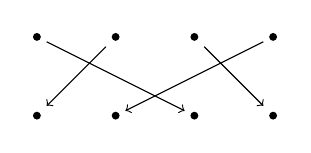
\begin{tikzpicture}
		\node (p1) at (0, 0) {};
		\fill (0, 0) circle (0.05);
		
		\node (p2) at (1, 0) {};
		\fill (1, 0) circle (0.05);
		
		\node (p3) at (2, 0) {};
		\fill (2, 0) circle (0.05);
		
		\node (p4) at (3, 0) {};
		\fill (3, 0) circle (0.05);
		
		\node (t1) at (0, 1) {};
		\fill (0, 1) circle (0.05);
		
		\node (t2) at (1, 1) {};
		\fill (1, 1) circle (0.05);
		
		\node (t3) at (2, 1) {};
		\fill (2, 1) circle (0.05);
		
		\node (t4) at (3, 1) {};
		\fill (3, 1) circle (0.05);
		
		\draw[<-] (p1) -- (t2);
		\draw[<-] (p2) -- (t4);
		\draw[<-] (p3) -- (t1);
		\draw[<-] (p4) -- (t3);
	\end{tikzpicture}
\end{center}

An advantage of this is that it becomes easy to visualize things such as composition of maps. Furthermore, inverses are easy to see as well.

\chapter{Week For Suffering}
\section{Lecture -- 9/16/2024}
\subsection{Warm-Up}
\begin{hw}
	Prove that $3\ZZ = \brc{k \in \ZZ : 3 \mid k}$ is a group with the $+$ operation.
\end{hw}
\begin{solution}
	First, we prove that there exists an identity. We observe that $3(0) = 0$, so we see that $0 \in 3\ZZ$. Furthermore, note that $0 + k = k$ for all $k \in \ZZ$. Thus, since $3\ZZ \subseteq \ZZ$, we note that $0$ is also the identity in $3\ZZ$.
	
	Next, we observe that for any $k \in 3\ZZ$, we observe that there exists $a \in \ZZ$ such that $3a = k$. Then, we observe that if we let $b = -a$, then we have $3b = -k$. Thus, we see that $-k \in 3\ZZ$ as well. Then, we see that $k + (-k) = 0$. Thus, it passes the inverse check.
	
	Finally, we note that $+$ is associative on $\ZZ$, and thus it follows that it is associative on $3\ZZ$ as well.
\end{solution}

\begin{hw}
	How to find new examples of groups?
\end{hw}
\begin{solution}
	We can look at existing groups, and then form subgroups from them.
\end{solution}

\subsection{Subgroups}
\begin{defn}
	A subgroup $H$ of a group $G$ is a group $H$ with a group operation $*$ restricted from $G$.
\end{defn}

\begin{example}[Restriction]
	Let us suppose some set $X$ with a function $f$ mapping $X$ to $\RR$. So, we have $f : X \rightarrow \RR$. Then, there are times where we are only interested in some subset $Y \subset X$. Then, we look at $f : Y \rightarrow \RR$.
	
	Then, we have two notations:
	\begin{itemize}
		\item $f : Y \rightarrow \RR$.
		\item $f \restriction Y$
	\end{itemize}
\end{example}

So, for example, let consider $G = (G, *)$. Then, we have $* : G \times G \rightarrow G$. Now, we restrict it to $* : H \times H \rightarrow H$. We note that we have to enforce mapping to $H$, since $H$ is in fact a group.

\begin{example}($n\ZZ$)
	Let us consider $(\ZZ, +)$. Then, let us look at $(3\ZZ, +)$. This is in fact a subgroup of $(\ZZ, +)$. From the warm-up, we see that $(3\ZZ, +)$ is in fact a group.
	
	More generally, let us consider $n \in \ZZ$. Then, $n\ZZ = \brc{k \in \ZZ : n \mid k}$. Then, it is a subgroup a subgroup of $(\ZZ, +)$.
\end{example}

\begin{example}(A Non-Example)
	Let us consider $(\ZZ, +)$. Let us consider $(\ZZ/3\ZZ, +)$. We note that $(\ZZ/3\ZZ, +)$ is a group. We also note that we have closure, and so we see that $(\ZZ/3\ZZ, +)$ is... a subgroup?
	
	However, we note that $+$ isn't the same operation as we have on $(\ZZ, +)$. Furthermore, we see that $\ZZ/3\ZZ \not\subseteq \ZZ$.
\end{example}

\begin{defn}[Subgroup Lattice]
	We define a subgroup lattice of a group $G$ to be:
	
	\begin{equation*}
		(\brc{e}, *) \subset \cdots (H, *) \subset (K, *) \cdots \subset (G, *)
	\end{equation*}

	On the left-hand side is the trivial subgroup, the smallest possible subgroup. Then, the largest subgroup is the group itself. And everything in-between is what we call proper subgroups.
\end{defn}

\begin{defn}[Proper Subgroup]
	Proper subgroups are subgroups which are not the group itself and not the trivial subgroup.
\end{defn}

\begin{prop}
	We say that $H \subseteq G$ is a subgroup if and only if:
	\begin{itemize}
		\item $e_G \in H$.
		\item If $h_1, h_2 \in H$, then $h_1h_2 \in H$.
		\item If $h \in H$, then $h^{-1} \in H$
	\end{itemize}
\end{prop}
\begin{proof}
	First, let us suppose that $H \subseteq G$ is a subgroup. Then, we'll prove that the three properties hold.
	\begin{innerproof}
		First, let us show that $e_G \in H$. We observe that since $H$ is a subgroup, we have that $e_H \in H$ and that for all $h \in H$, we have $e_H h = h e_H = h$.
		
		Furthermore, we note that $e_H \in G$, so we see that $e_G e_H = e_H e_G = e_H$.
		
		Now, we observe the following:
		\begin{align*}
			e_G e_H = e_H e_G = e_H
		\end{align*}
	
		Furthermore, we have:
		\begin{align*}
			e_H e_H = e_H
		\end{align*}
	
		So, we have:
		\begin{align*}
			e_G e_H &= e_H e_H \\
			e_G (e_H e_H^{-1}) &= e_H(e_H e_H^{-1}) \\
			e_G &= e_H
		\end{align*}
	
		Next, let us consider inverses. Since $H$ is a subgroup, we know then that if $h \in H$, we have an inverse $h'$ such that $hh' = h'h = e$. And we note by the uniqueness of inverses in $G$, we have that $h' = h^{-1}$.
		
		Finally, for closure, we note that it follows from the fact that $H$ is in fact a group.
	\end{innerproof}
\end{proof}

\begin{prop}
	$H \subseteq G$ is a subgroup if and only if $H \neq \emptyset$ and $\forall a, b \in H$, we have $ab^{-1} \in H$.
\end{prop}
\begin{solution}
	First, let us show that if $H \neq \emptyset$ and $\forall a,b \in H$, we have $ab^{-1} \in H$, then we have $H$ is a subgroup.
	\begin{innerproof}
		First, since $H \neq \emptyset$, let us then consider $h \in H$. Then, $hh = hh^{-1} = e \in H$.
		
		Next, let us consider $h \in H$. Then, we observe that since we know $e \in H$, we have that $eh^{-1} = h^{-1} \in H$.
		
		Finally, let us consider $h_1, h_2 \in H$. We want to show that $h_1 h_2 \in H$ (i.e. we have closure). Since $H$ respects inverses, we see that if $h_2 \in H$, we have $h_2^{-1} \in H$ as well.
		
		Then, we see that $h_1, h_2^{-1} \in H$. Then, we have $h_1(h_2^{-1})^{-1} = h_1h_2\in H$.
		
		Therefore, we note that $H$ is in fact a subgroup.
	\end{innerproof}
	
\end{solution}

\end{document}